\documentclass[border=4pt]{standalone}
% Preámbulo común de las figuras. Cada figura es un documento standalone
% que se compila a SVG con scripts/build_figures.sh
\usepackage[utf8]{inputenc}
\usepackage{amsmath}
\usepackage{tikz}
\usepackage[american, siunitx]{circuitikz}
\usetikzlibrary{arrows.meta,calc,decorations.pathmorphing,patterns}
\tikzset{
  >={Stealth[length=2.2mm]},
  eje/.style={->, thin},
  hilo/.style={thick},
}
% Paleta común: tonos medios legibles sobre fondo claro
\definecolor{azul}{RGB}{31,94,168}
\definecolor{rojo}{RGB}{192,57,43}
\definecolor{verde}{RGB}{39,128,73}
\definecolor{naranja}{RGB}{211,120,30}
\definecolor{morado}{RGB}{125,60,152}

\begin{document}
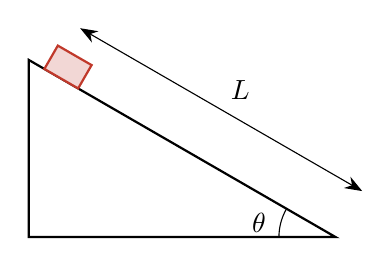
\begin{tikzpicture}[scale=0.9]
  % techo de 30 grados: base 4.33, altura 2.5
  \draw[thick] (0,0) -- (4.33,0) -- (0,2.5) -- cycle;
  \draw (3.53,0) arc (180:150:0.8); \node at (3.25,0.2) {$\theta$};
  \begin{scope}[shift={(0.35,2.298)}, rotate=-30]
    \filldraw[draw=rojo, fill=rojo!20, thick] (-0.15,0) rectangle (0.4,0.38);
  \end{scope}
  \draw[<->, thin] ($(0.35,2.298)+(60:0.75)$) -- node[above right]{$L$} ($(4.33,0)+(60:0.75)$);
\end{tikzpicture}
\end{document}
